\documentclass[a4paper, 14pt]{extarticle}
\usepackage[russian]{babel}
\usepackage[T1]{fontenc}
\usepackage{fontspec}
\usepackage{indentfirst}
\usepackage{enumitem}
\usepackage{graphicx}
\usepackage[
  left=20mm,
  right=10mm,
  top=20mm,
  bottom=20mm
]{geometry}
\usepackage{parskip}
\usepackage{titlesec}
\usepackage{xurl}
\usepackage{hyperref}
\usepackage{float}
\usepackage[
  figurename=Рисунок,
  labelsep=endash,
]{caption}
\usepackage[outputdir=build, newfloat]{minted}
\usepackage{multirow}
\usepackage{array}

\hypersetup{
  colorlinks=true,
  linkcolor=black,
  filecolor=blue,
  urlcolor=blue,
}

\renewcommand*{\labelitemi}{---}
\setmainfont{Times New Roman}
\setmonofont{JetBrains Mono}[
  SizeFeatures={Size=11},
]

\newenvironment{code}{\captionsetup{type=listing}}{}
\SetupFloatingEnvironment{listing}{name=Листинг}

\setminted{
  fontsize=\footnotesize,
  framesep=0mm,
}

\captionsetup{width=\textwidth,justification=centering}
\captionsetup[table]{singlelinecheck=off,justification=justified}

\newcolumntype{L}[1]{>{\raggedright\let\newline\\\arraybackslash\hspace{0pt}}m{#1}}
\newcolumntype{C}[1]{>{\centering\let\newline\\\arraybackslash\hspace{0pt}}m{#1}}
\newcolumntype{R}[1]{>{\raggedleft\let\newline\\\arraybackslash\hspace{0pt}}m{#1}}

\setlength{\parskip}{6pt}

\setlength{\parindent}{1cm}
\setlist[itemize]{itemsep=0em,topsep=0em,parsep=0em,partopsep=0em,leftmargin=2.0cm}
\setlist[enumerate]{itemsep=0em,topsep=0em,parsep=0em,partopsep=0em,leftmargin=2.0cm}

\renewcommand{\thesection}{\arabic{section}.}
\renewcommand{\thesubsection}{\thesection\arabic{subsection}.}
\renewcommand{\thesubsubsection}{\thesubsection\arabic{subsubsection}.}

\titleformat{\section}{\normalfont\bfseries}{\thesection}{0.5em}{}
\titleformat{\subsection}{\normalfont\bfseries}{\thesubsection}{0.5em}{}

\titleformat*{\section}{\normalfont\bfseries}
\titleformat*{\subsection}{\normalfont\bfseries}

\linespread{1.5}
\renewcommand{\baselinestretch}{1.5}
\begin{document}

\begin{titlepage}
  \vspace{0pt plus2fill}
  \noindent

  \vspace{0pt plus6fill}
  \begin{center}
    Санкт-Петербургский национальный исследовательский университет
    информационных технологий, механики и оптики

    \vspace{0pt plus3fill}

    Факультет инфокоммуникационных технологий

    Направление подготовки 11.03.02

    \vspace{0pt plus2fill}

    Практическая работа №3

    \vspace{0pt plus1fill}

    Изучение работы концентраторов и коммутаторов.

    Организация виртуальных сетей. DHCP-сервер.

  \end{center}

  \vspace{0pt plus7fill}
  \begin{flushright}
    Выполнил: \\
    Швалов Даниил Андреевич

    Группа: К33211

    Проверил: \\
    Харитонов Антон
  \end{flushright}

  \vspace{0pt plus2fill}
  \begin{center}
    Санкт-Петербург

    2023
  \end{center}
\end{titlepage}

\setcounter{page}{2}

\section{Введение}

\textbf{Цель работы}: изучить и практически ознакомиться с основными принципами
работы концентраторов и коммутаторов второго уровня в компьютерных сетях, а
также настроить и использовать DHCP-сервер для автоматической выдачи IP-адресов
в локальной сети.

\section{Тестирование работы концентратора в среде моделирования Cisco Packet Tracer}

В качестве сети, в которой будут работать заданные 6 устройств, была выбрана
сеть №3 из лабораторной работы №2. Таким образом, все устройства будут
находиться в подсети \texttt{192.168.32.0/22}. Согласно описанию все устройства
были добавлены на схему (рис. \ref{fig:task-1:scheme-1}). После этого все
компьютеры были подключены к коммутатору (рис. \ref{fig:task-1:scheme-2}).

\begin{figure}[H]
  \centering
  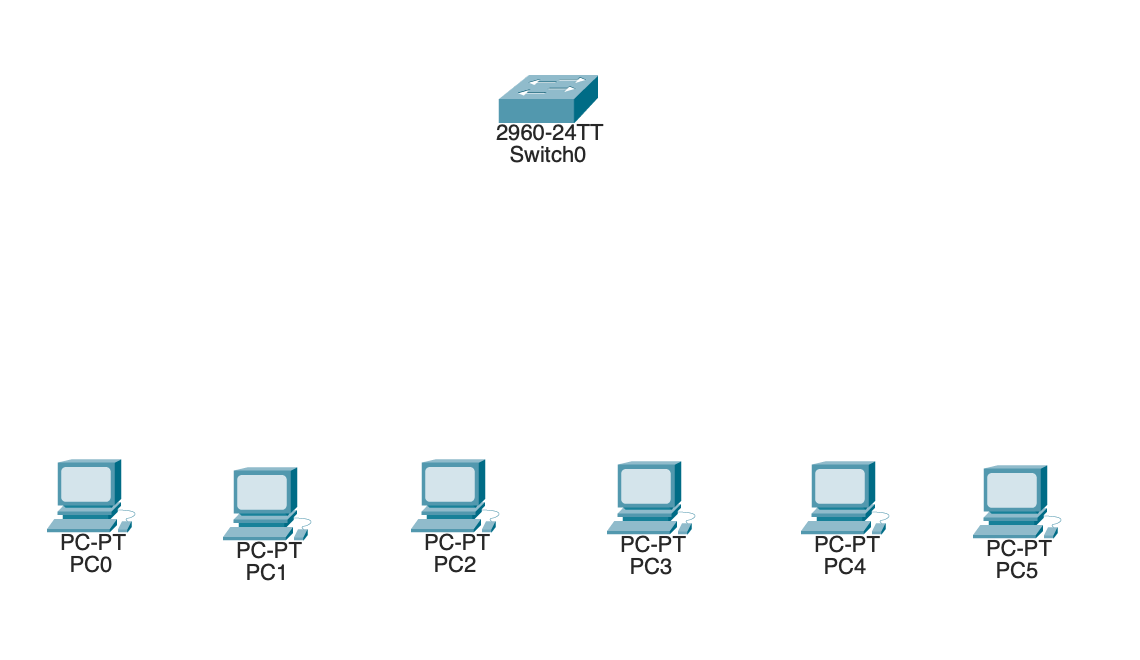
\includegraphics[width=0.8\textwidth]{images/task-1/scheme-1.png}
  \caption{Схема сети}
  \label{fig:task-1:scheme-1}
\end{figure}

\begin{figure}[H]
  \centering
  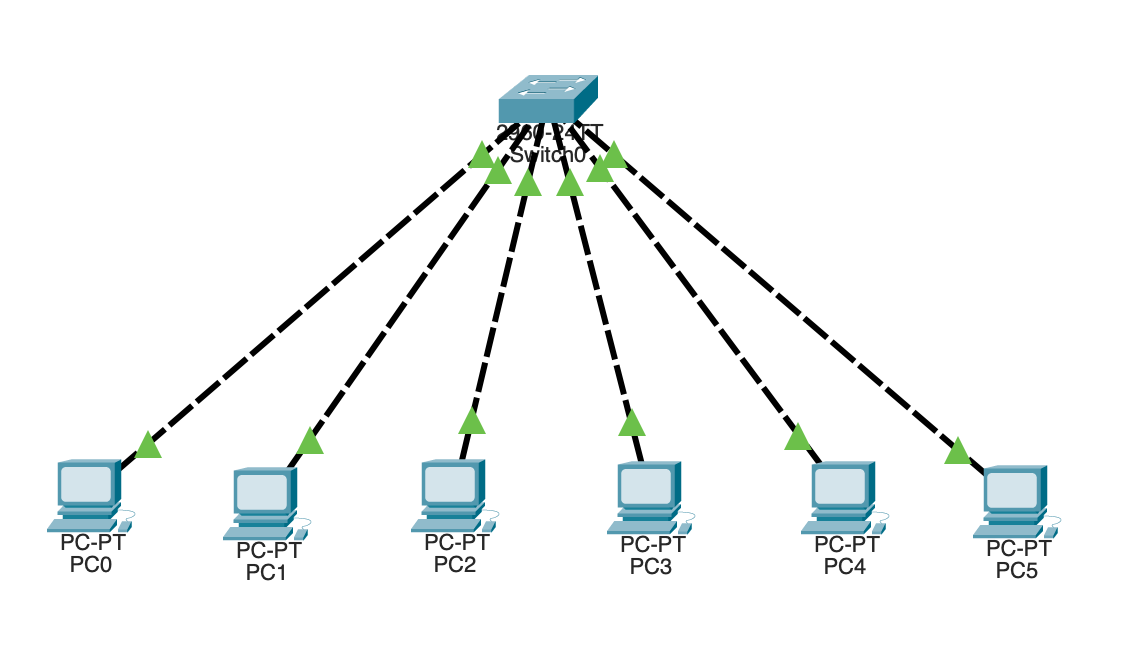
\includegraphics[width=0.8\textwidth]{images/task-1/scheme-2.png}
  \caption{Схема сети}
  \label{fig:task-1:scheme-2}
\end{figure}

После подключения на всех компьютерах был настроен IP-адрес устройства (рис.
\ref{fig:task-1:ip-config}). В таблице \ref{tab:task-1:ip-config} приведено
описание всех компьютеров и их адресов.

\begin{figure}[H]
  \centering
  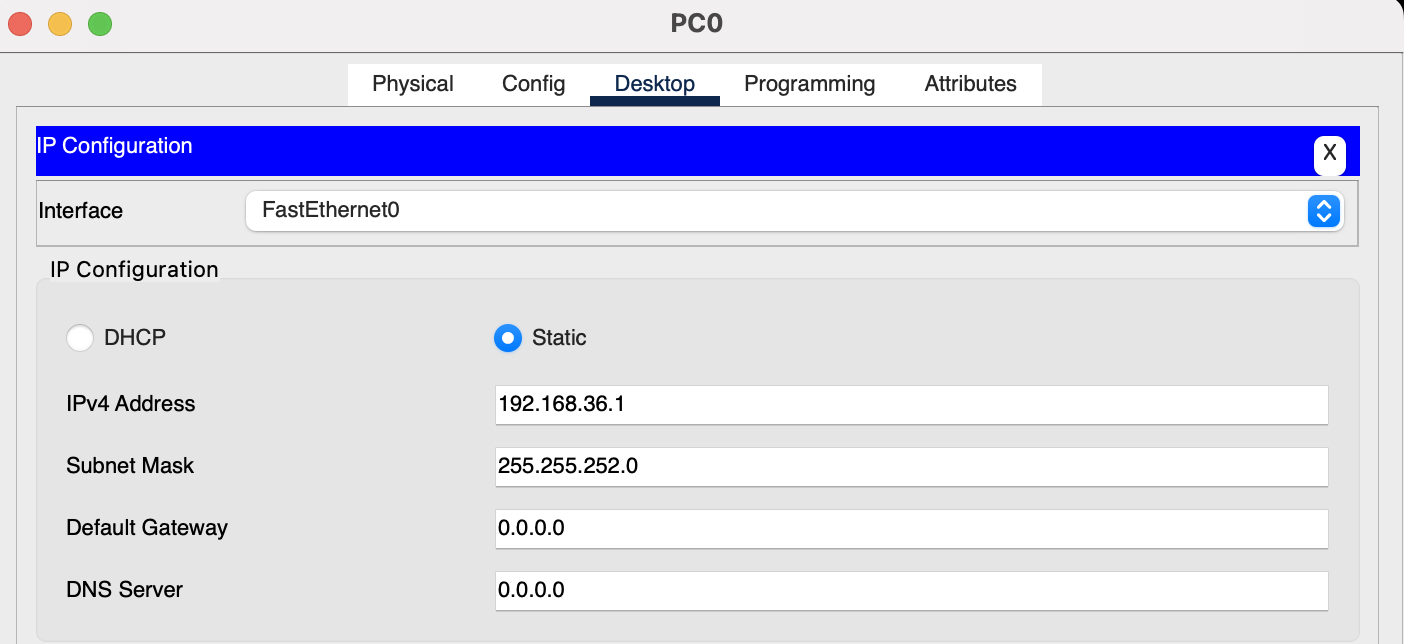
\includegraphics[width=\textwidth]{images/task-1/ip-config.png}
  \caption{Настройка IP-адреса компьютера PC0}
  \label{fig:task-1:ip-config}
\end{figure}

\begin{table}[H]
  \centering
  \caption{IP адреса компьютеров}
  \label{tab:task-1:ip-config}

  \setlength{\tabcolsep}{12pt}
  \renewcommand*{\arraystretch}{1.5}

  \begin{tabular}{|c|c|c|c|}
    \hline
    \textbf{Название} & \textbf{IP-адрес} & \textbf{Название} & \textbf{IP-адрес} \\
    \hline
    PC0               & 192.168.32.1      & PC3               & 192.168.32.4      \\
    \hline
    PC1               & 192.168.32.2      & PC4               & 192.168.32.5      \\
    \hline
    PC2               & 192.168.32.3      & PC5               & 192.168.32.6      \\
    \hline
  \end{tabular}
\end{table}

Чтобы протестировать получившуюся сеть, использовался режим симуляции в CPT.
Так, с помощью простого PDU был отправлен ICMP запрос с компьютера PC0 на
компьютер PC4 (рис. \ref{fig:task-1:arp-1}). Поскольку изначально компьютер PC0
не знает MAC-адрес компьютера PC4, компьютер PC0 совершает ARP запрос (рис.
\ref{fig:task-1:arp-2}). Поскольку коммутатор не настроен на фильтрацию пакетов,
он рассылает ARP-запрос сразу всем подключенным к нему компьютерам (рис.
\ref{fig:task-1:arp-3}). После того, как компьютер PC0 выяснил MAC-адрес
компьютера PC4 (рис. \ref{fig:task-1:arp-4}-\ref{fig:task-1:arp-5}), ICMP-запрос
был успешно доставлен до адресата, равно как и ICMP-ответ (рис.
\ref{fig:task-1:pdu-1}-\ref{fig:task-1:pdu-4}).

\begin{figure}[H]
  \centering
  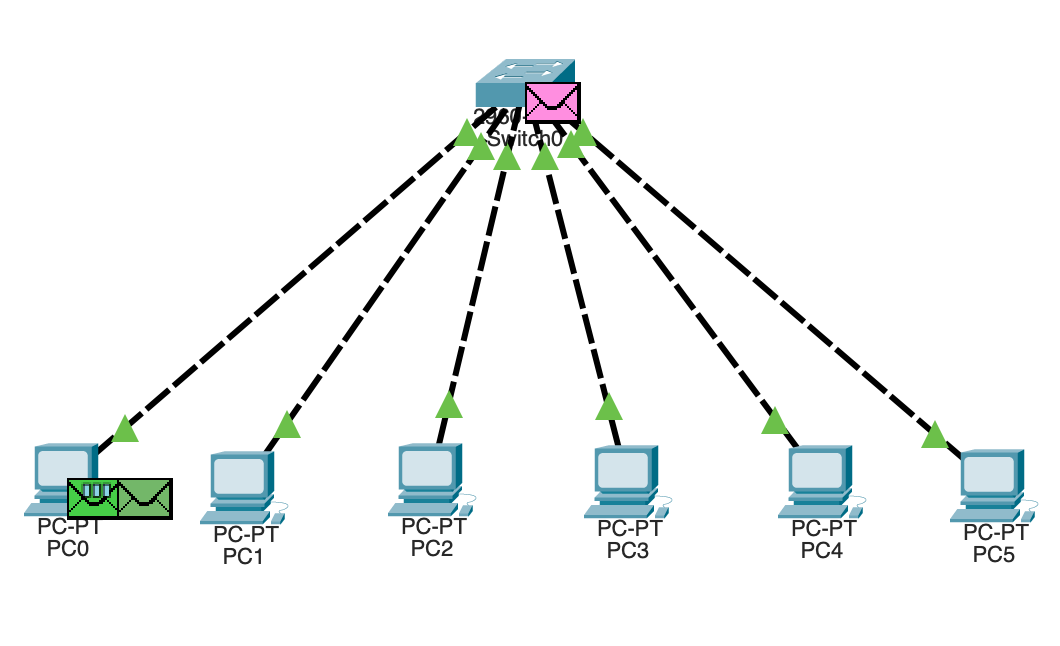
\includegraphics[width=0.8\textwidth]{images/task-1/arp-1.png}
  \caption{ARP-запрос}
  \label{fig:task-1:arp-1}
\end{figure}

\begin{figure}[H]
  \centering
  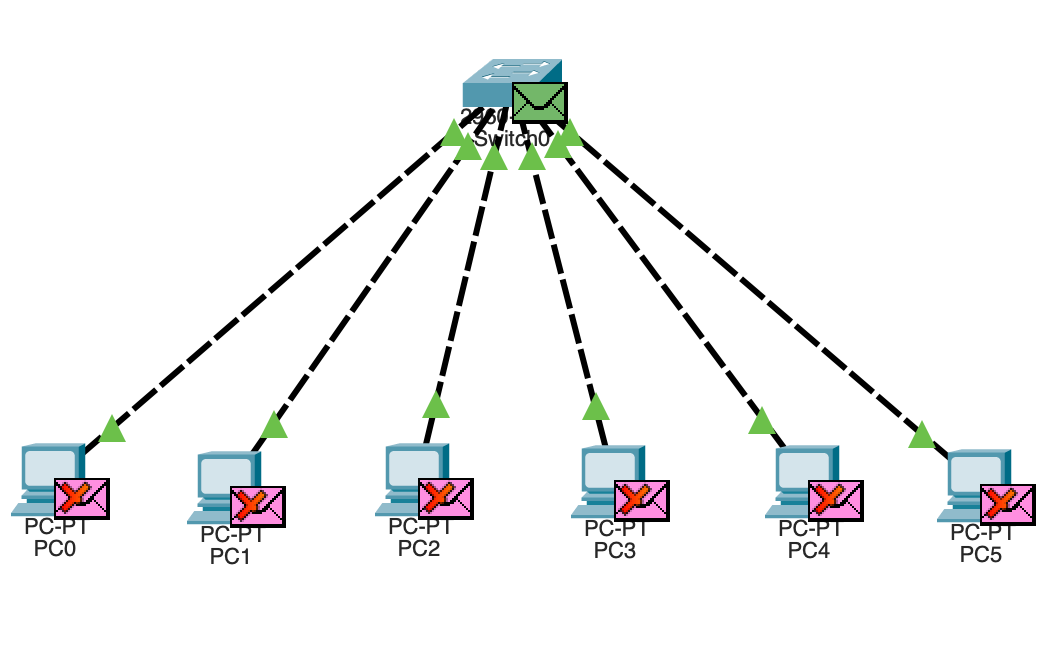
\includegraphics[width=0.8\textwidth]{images/task-1/arp-2.png}
  \caption{ARP-запрос}
  \label{fig:task-1:arp-2}
\end{figure}

\begin{figure}[H]
  \centering
  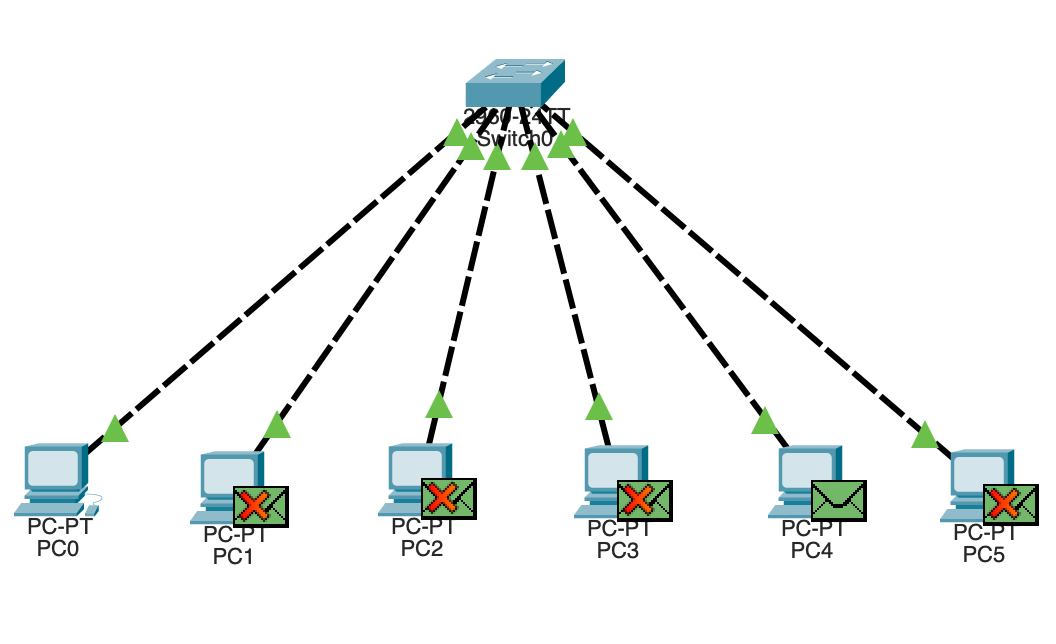
\includegraphics[width=0.8\textwidth]{images/task-1/arp-3.png}
  \caption{ARP-запрос}
  \label{fig:task-1:arp-3}
\end{figure}

\begin{figure}[H]
  \centering
  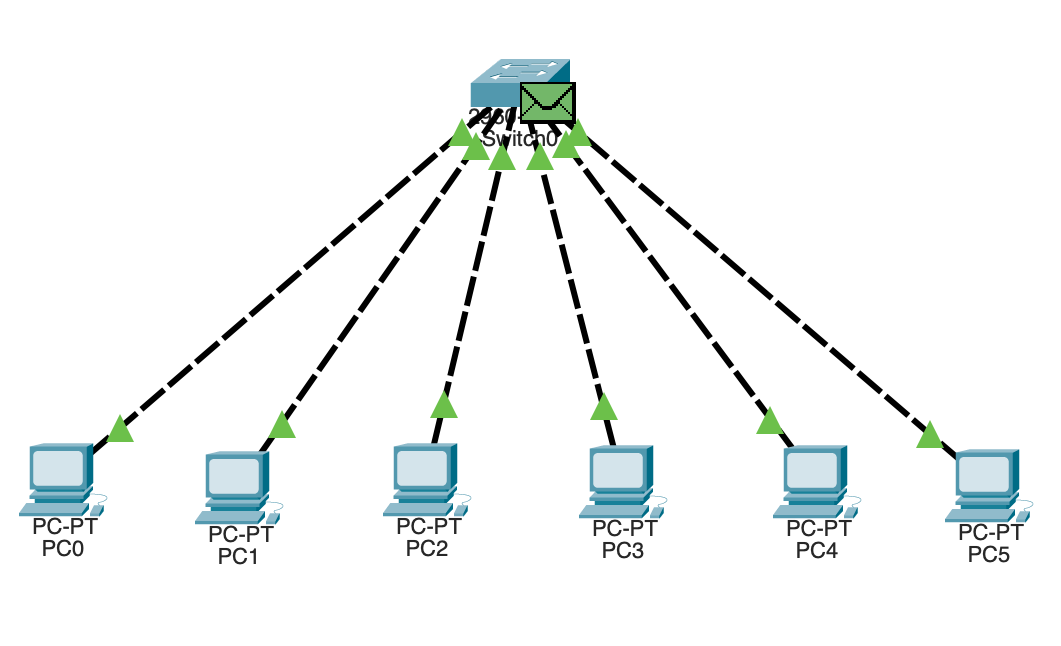
\includegraphics[width=0.8\textwidth]{images/task-1/arp-4.png}
  \caption{ARP-запрос}
  \label{fig:task-1:arp-4}
\end{figure}

\begin{figure}[H]
  \centering
  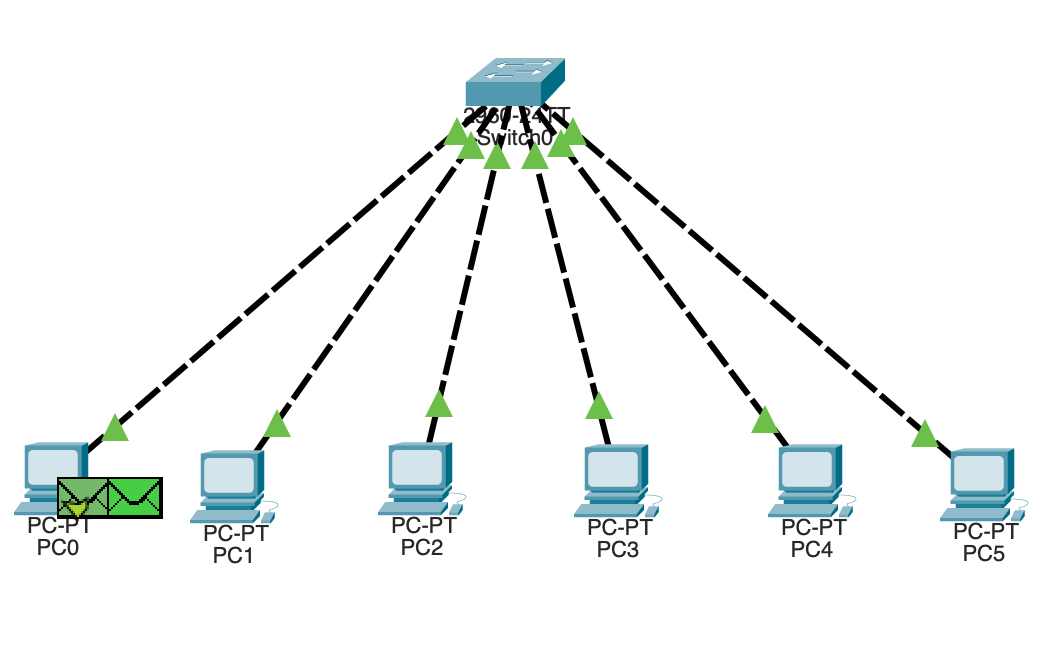
\includegraphics[width=0.8\textwidth]{images/task-1/arp-5.png}
  \caption{ARP-запрос}
  \label{fig:task-1:arp-5}
\end{figure}

\begin{figure}[H]
  \centering
  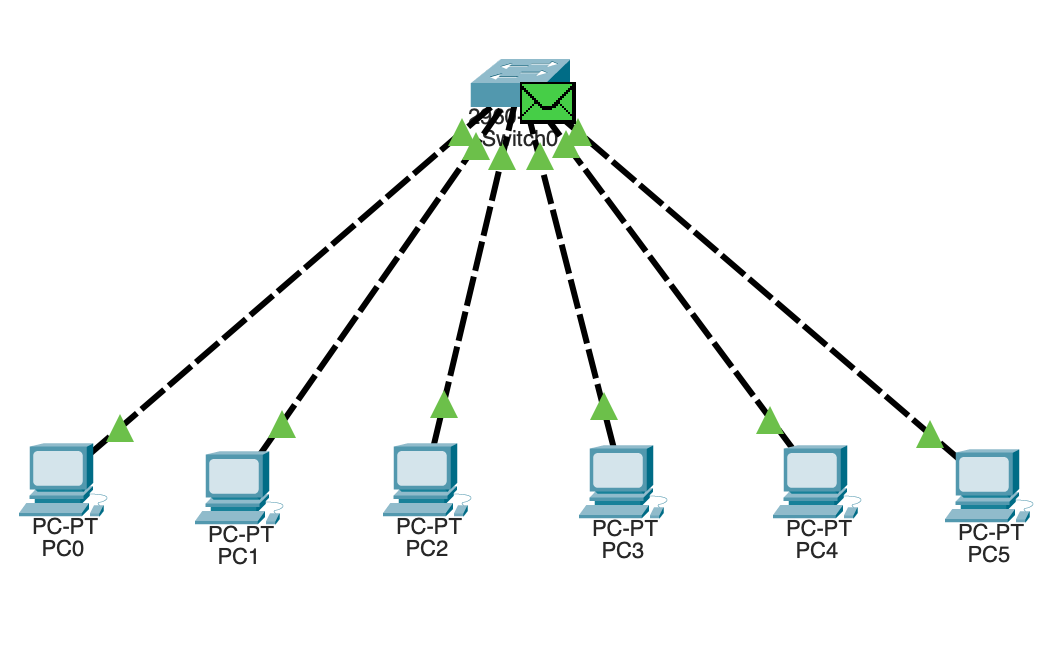
\includegraphics[width=0.8\textwidth]{images/task-1/pdu-1.png}
  \caption{ICMP-запрос}
  \label{fig:task-1:pdu-1}
\end{figure}

\begin{figure}[H]
  \centering
  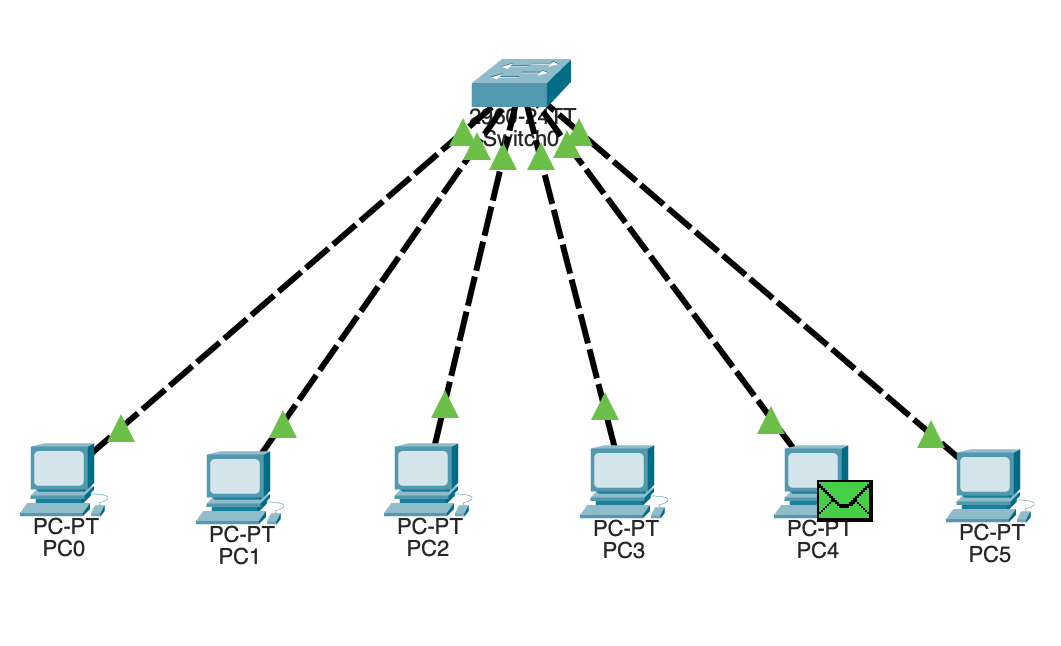
\includegraphics[width=0.8\textwidth]{images/task-1/pdu-2.png}
  \caption{ICMP-запрос}
  \label{fig:task-1:pdu-2}
\end{figure}

\begin{figure}[H]
  \centering
  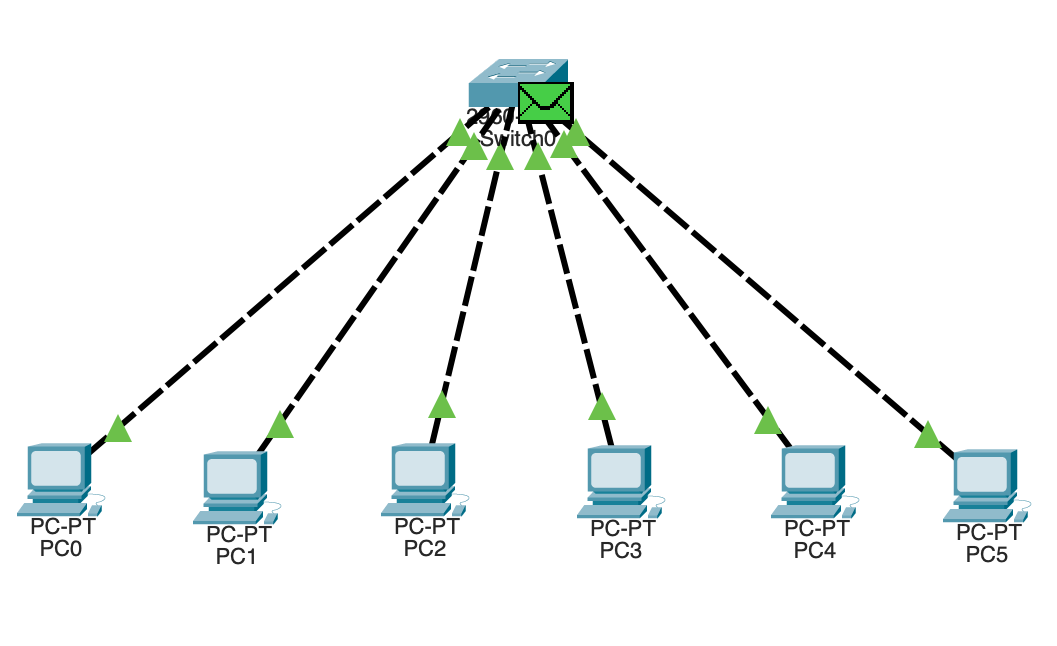
\includegraphics[width=0.8\textwidth]{images/task-1/pdu-3.png}
  \caption{ICMP-запрос}
  \label{fig:task-1:pdu-3}
\end{figure}

\begin{figure}[H]
  \centering
  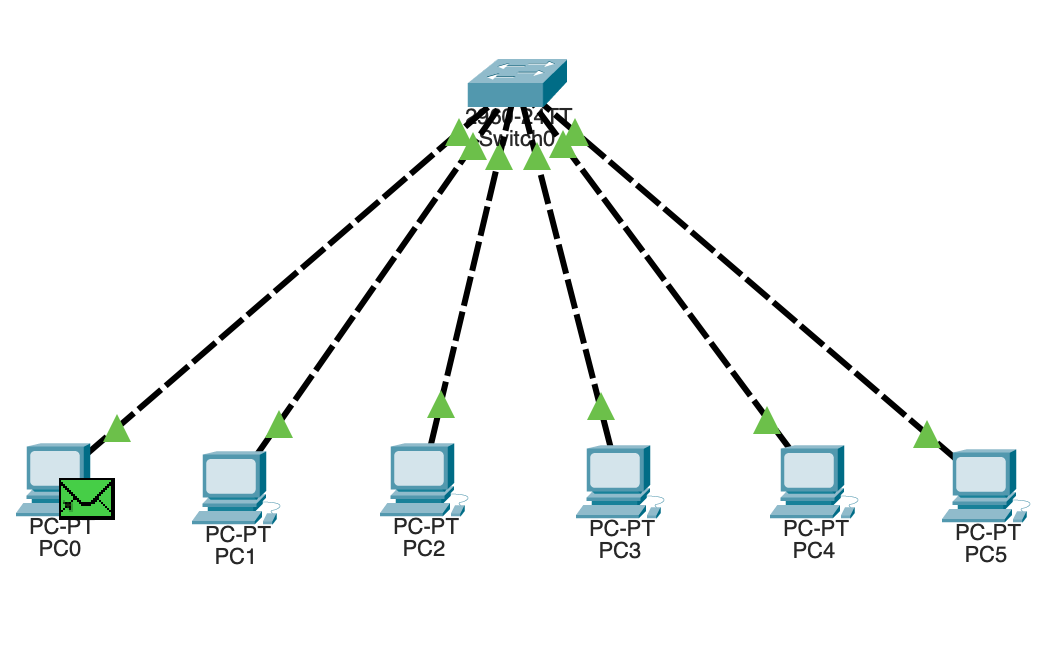
\includegraphics[width=0.8\textwidth]{images/task-1/pdu-4.png}
  \caption{ICMP-запрос}
  \label{fig:task-1:pdu-4}
\end{figure}

\section{Организация и моделирование виртуальных сетей}

Согласно заданию, в каждом помещении было расположено соответствующее количество
устройств (рис. \ref{fig:task-2:physical-1}). Поскольку в прошлой лабораторной
работе в первой сети было пять подсетей, во второй сети было три подсети, а в
третьей сети было также пять подсетей, значит, в этом задании необходимо создать
три подсети с компьютерами, три подсети с принтерами, две подсети с
IP-телефонами, две подсети с веб-камерами и две подсети с ноутбуками. На рис.
\ref{fig:task-2:logical-1} показана логическая схема сети, в которой каждая
подсеть отмечена отдельным цветом.

\begin{figure}[H]
  \centering
  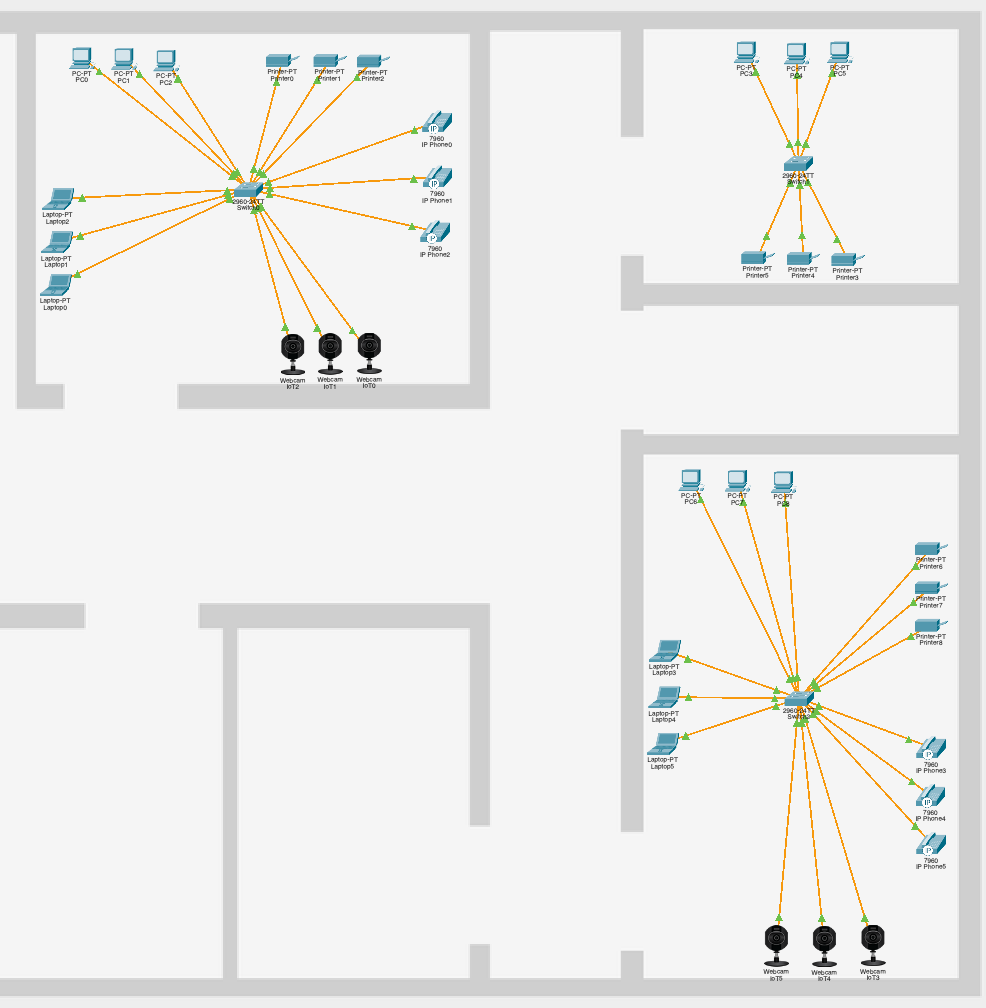
\includegraphics[width=\textwidth]{images/task-2/physical-1.png}
  \caption{Схема физического расположения устройств}
  \label{fig:task-2:physical-1}
\end{figure}

\begin{figure}[H]
  \centering
  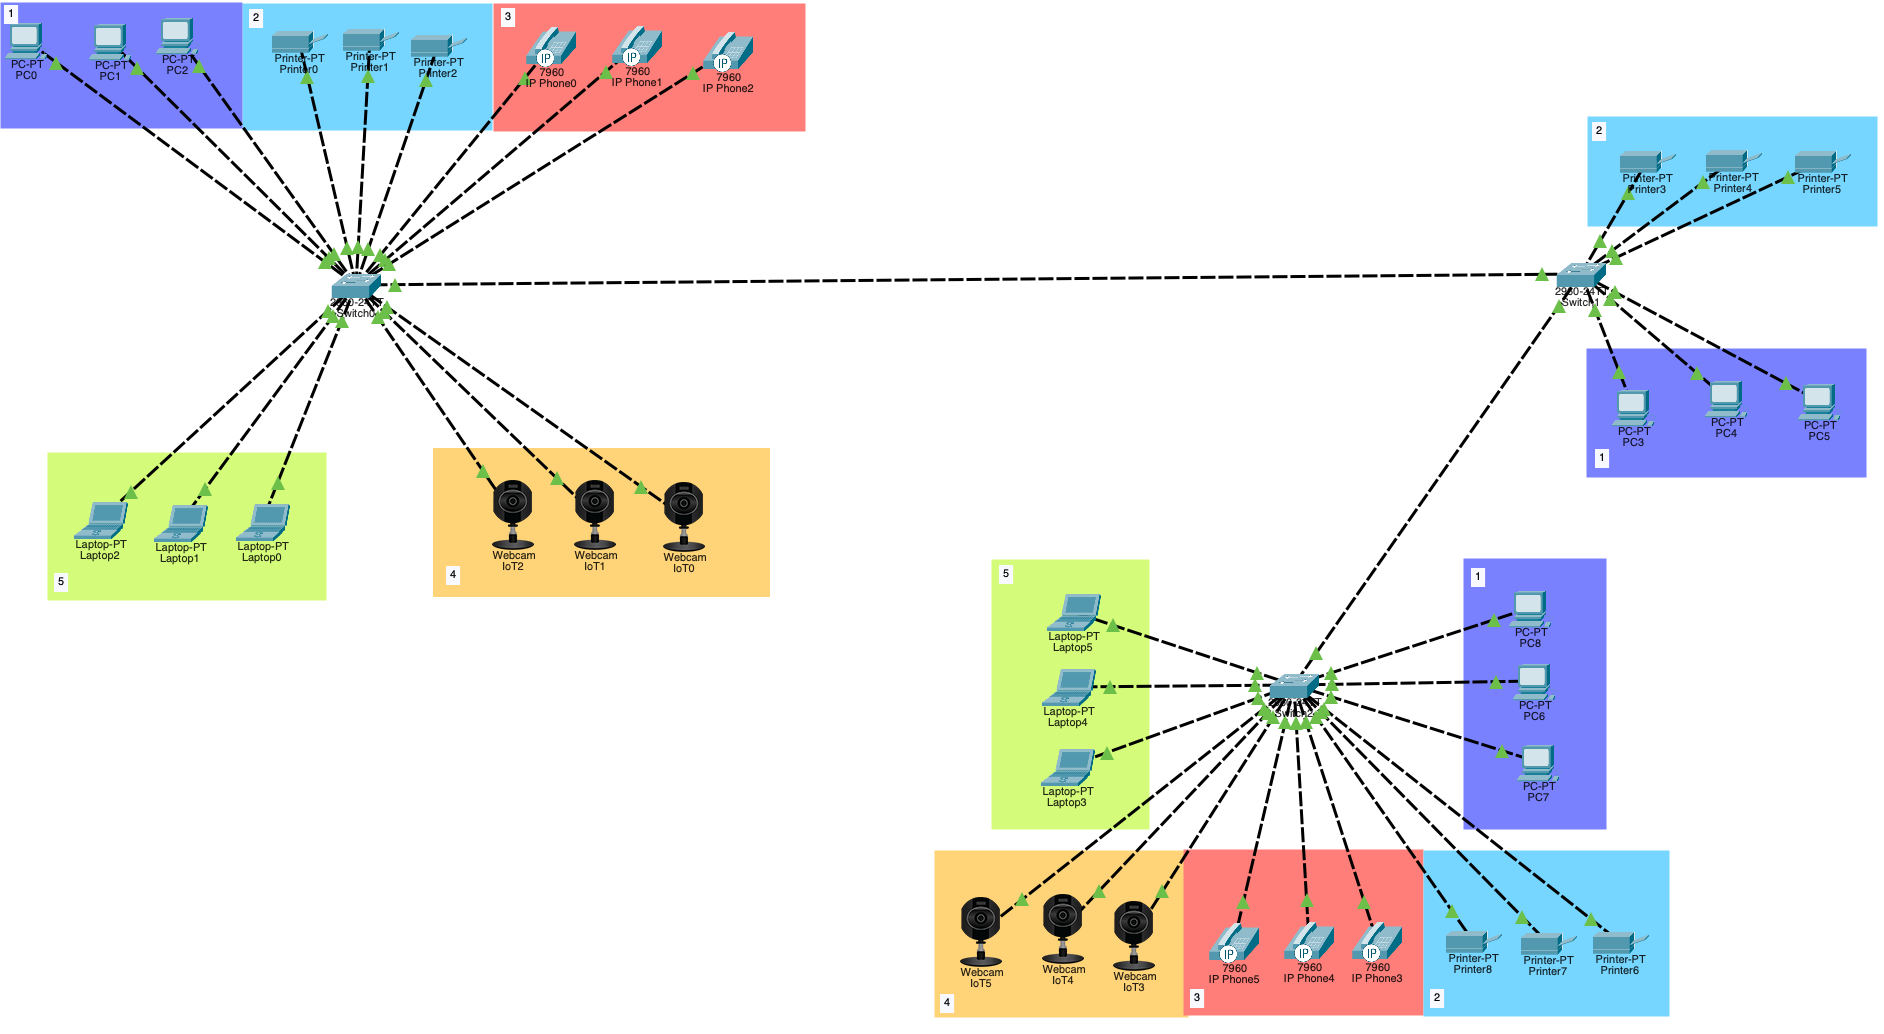
\includegraphics[width=\textwidth]{images/task-2/logical-1.png}
  \caption{Логическая схема}
  \label{fig:task-2:logical-1}
\end{figure}

После добавления всех конечных устройств, была произведена настройка
коммутаторов. Сначала для всех коммутаторов была добавлена информация о всех
существующих VLAN с помощью команды \texttt{vlan N}, где \texttt{N} --- номер
каждого VLAN. Затем на каждом из коммутаторов были настроены VLAN с помощью
следующих команд (на примере интерфейса FastEthernet0/1):
\begin{minted}{text}
  interface FastEthernet0/1
  switchport access vlan 10
\end{minted}
Так было проделано для всех портов, которые используются для конченых устройств.
Для всех портов, которые соединяются с другими промежуточными сетевыми
устройствами, использовались следующие команды для настройки (на примере
интерфейса FastEthernet0/23):
\begin{minted}{text}
  interface FastEthernet0/23
  switchport mode trunk
\end{minted}

После настройки всех коммутаторов были добавлены коммутатор третьего уровня и
сервер, который будет выступать в качестве DCHP сервера (рис.
\ref{fig:task-2:physical-2} и \ref{fig:task-2:logical-2}).

\begin{figure}[H]
  \centering
  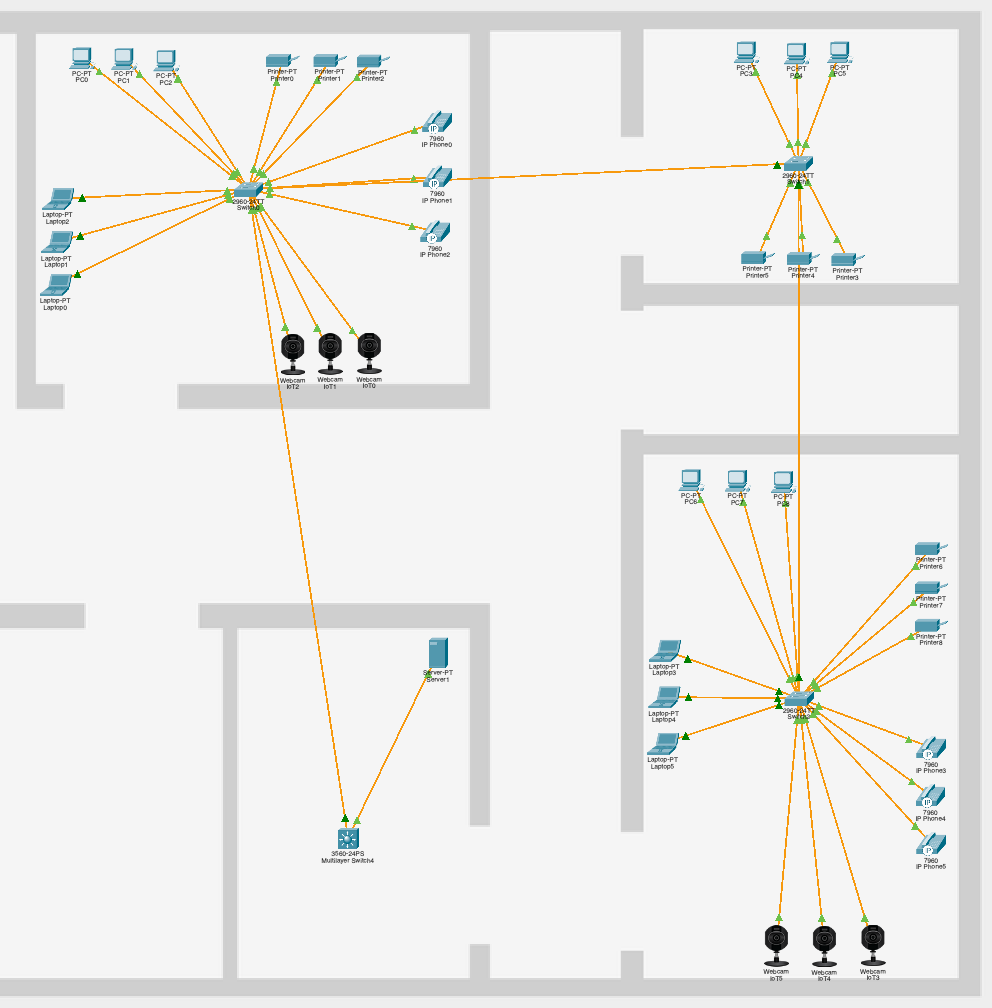
\includegraphics[width=\textwidth]{images/task-2/physical-2.png}
  \caption{Схема физического расположения устройств}
  \label{fig:task-2:physical-2}
\end{figure}

\begin{figure}[H]
  \centering
  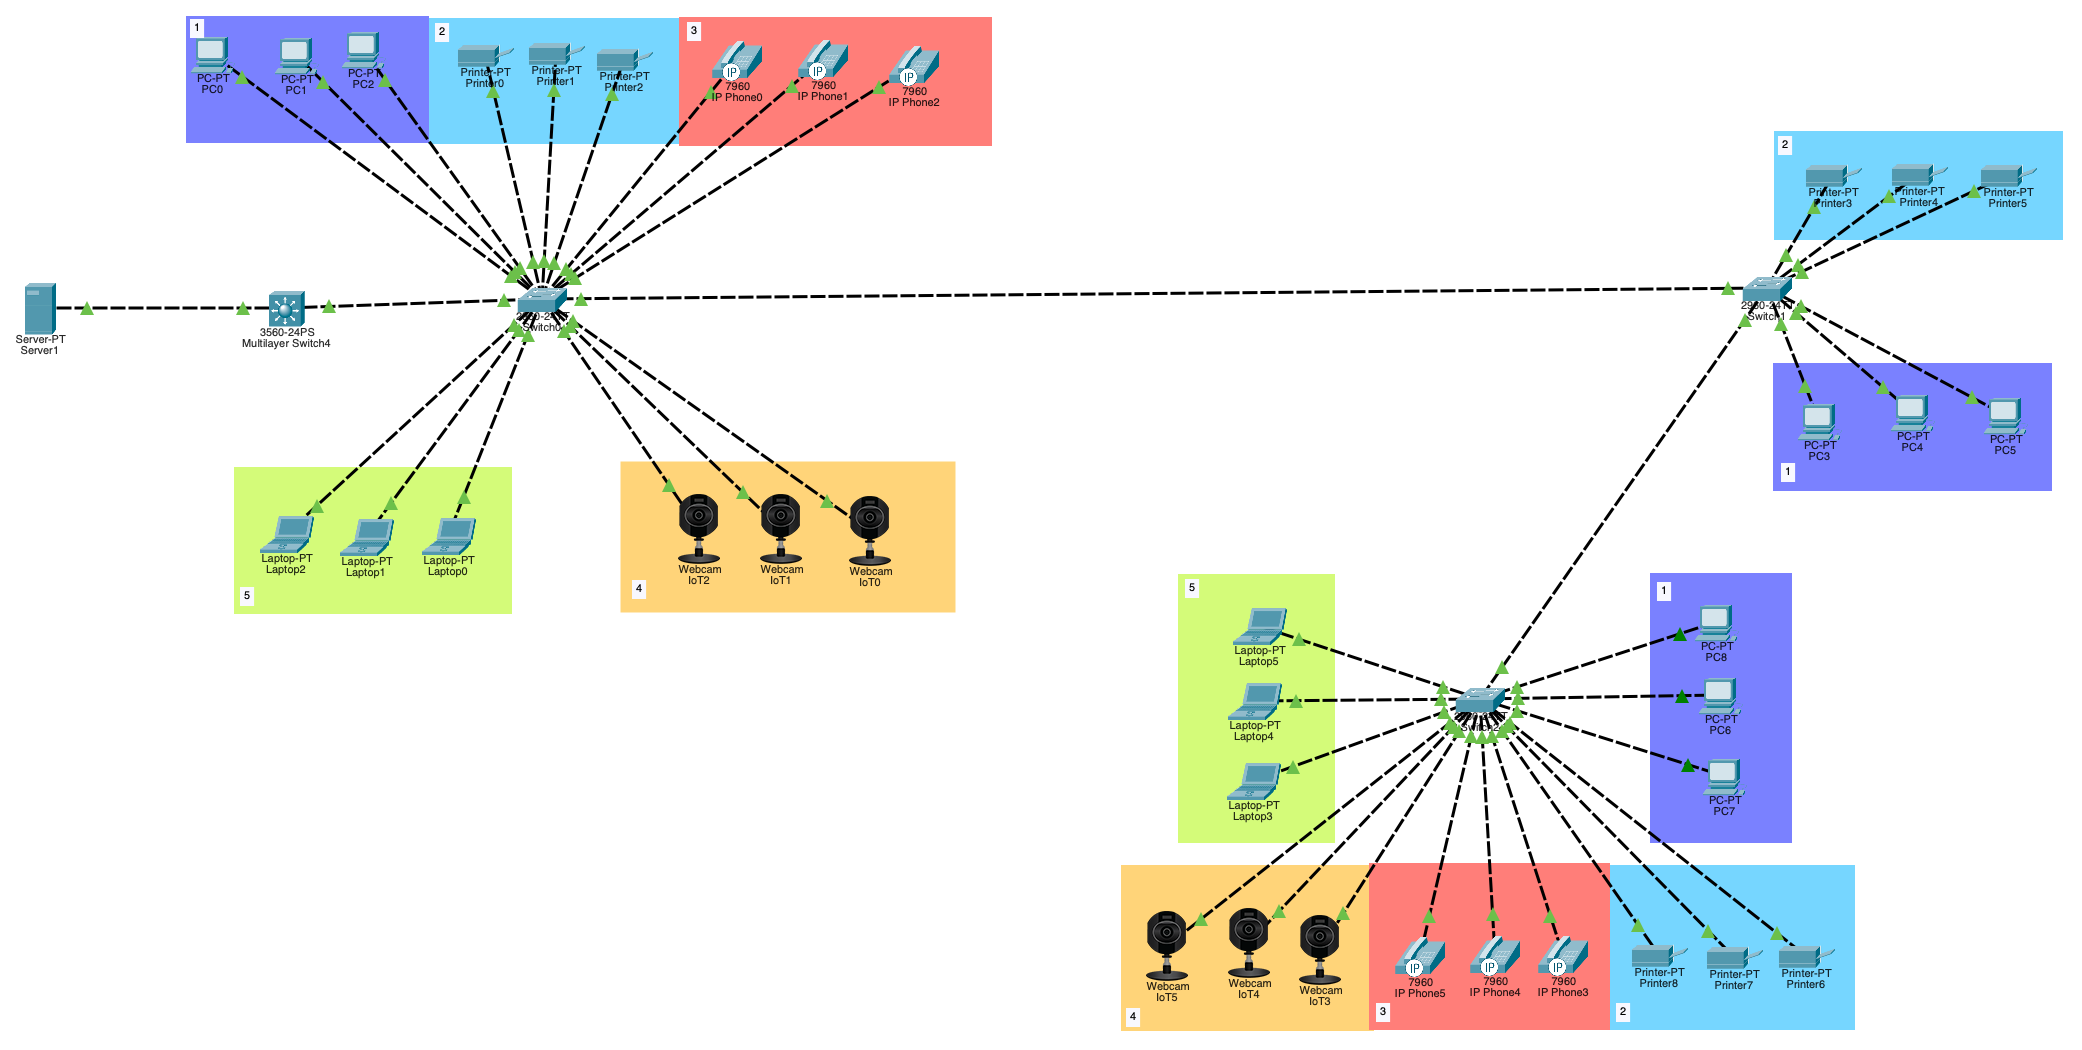
\includegraphics[width=\textwidth]{images/task-2/logical-2.png}
  \caption{Логическая схема}
  \label{fig:task-2:logical-2}
\end{figure}

В настройках сервера был включен и настроен DHCP сервер. На рис.
\ref{fig:task-2:dhcp-config} показаны итоговые настройки DHCP сервера.

\begin{figure}[H]
  \centering
  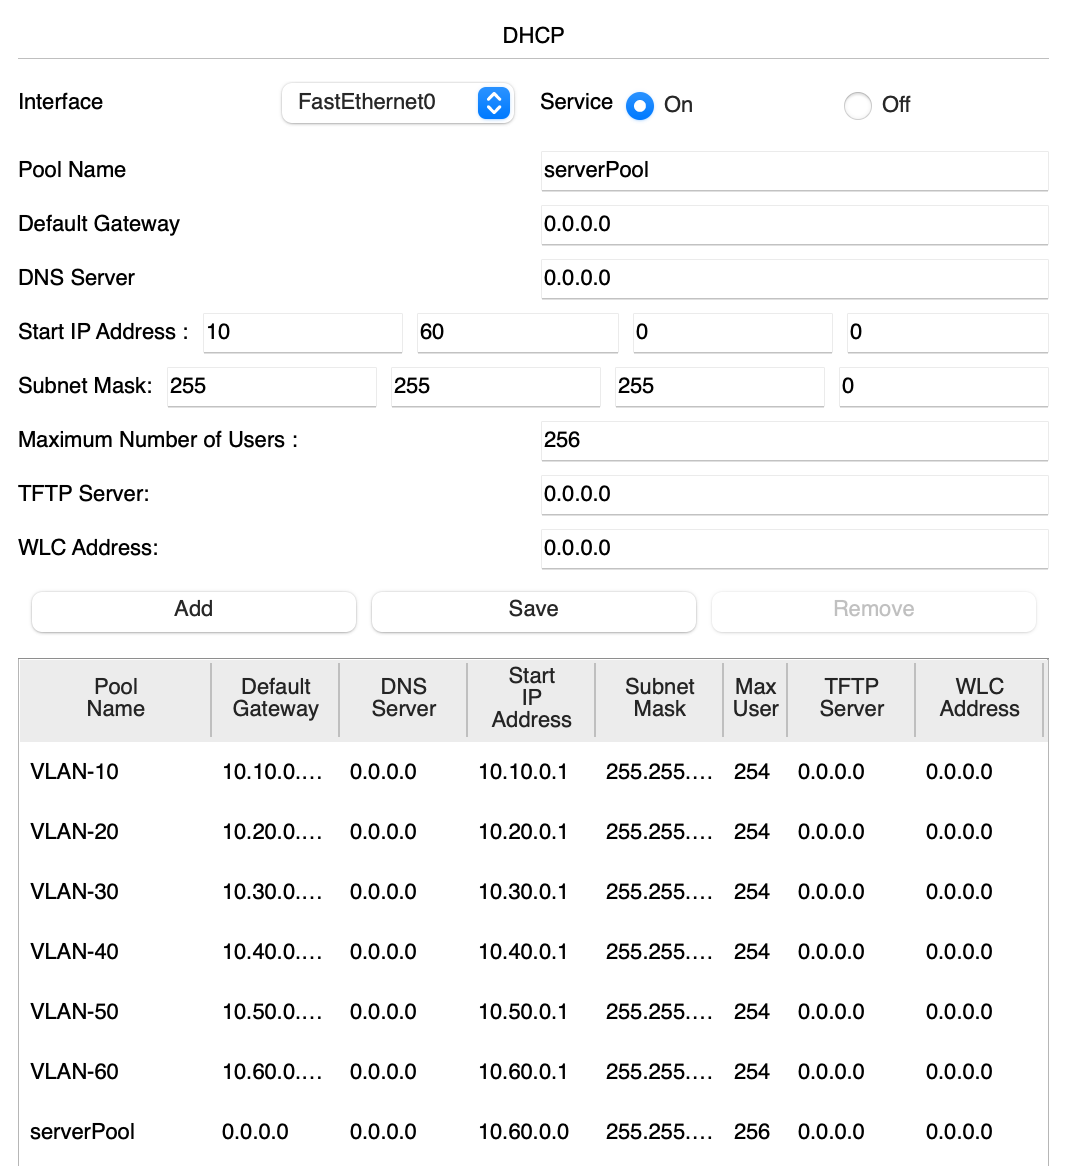
\includegraphics[width=0.55\textwidth]{images/task-2/dhcp-config.png}
  \caption{Настройки DHCP сервера}
  \label{fig:task-2:dhcp-config}
\end{figure}

После настройки DHCP сервера была произведена настройка коммутатора третьего
уровня. С помощью команды \texttt{vlan database} и команды \texttt{vlan N}, где
\texttt{N} --- номер каждого VLAN, в коммутатор была добавлена информация о всех
существующих VLAN. Затем для каждого VLAN с помощью команд (на примере VLAN 10)
\begin{minted}{text}
  interface vlan 10
  ip address 10.10.0.254 255.255.255.0
  ip helper-address 10.60.0.1
\end{minted}
была произведена настройка IP-адресов данных VLAN. После этого для порта, в
который подключен другой коммутатор, была произведена следующая настройка,
включающая режим trunk:
\begin{minted}{text}
  interface FastEthernet0/2
  switchport trunk encapsulation dot1q
  switchport mode trunk
\end{minted}
Затем была произведена настройка порта, в который подключен DHCP сервер.
Поскольку сервер находится в VLAN 60, были выполнены следующие команды:
\begin{minted}{text}
  interface FastEthernet0/1
  switchport access vlan 10
\end{minted}

На этом настройка была завершена. Для тестирования работоспособности DHCP
сервера был выбран компьютер, на котором было настроено получение IP-настроек с
помощью DHCP сервера. После включения этой настройки DCHP сервер был успешно
найден, и компьютер получил свой IP-адрес (рис. \ref{fig:task-2:dhcp-request}).

\begin{figure}[H]
  \centering
  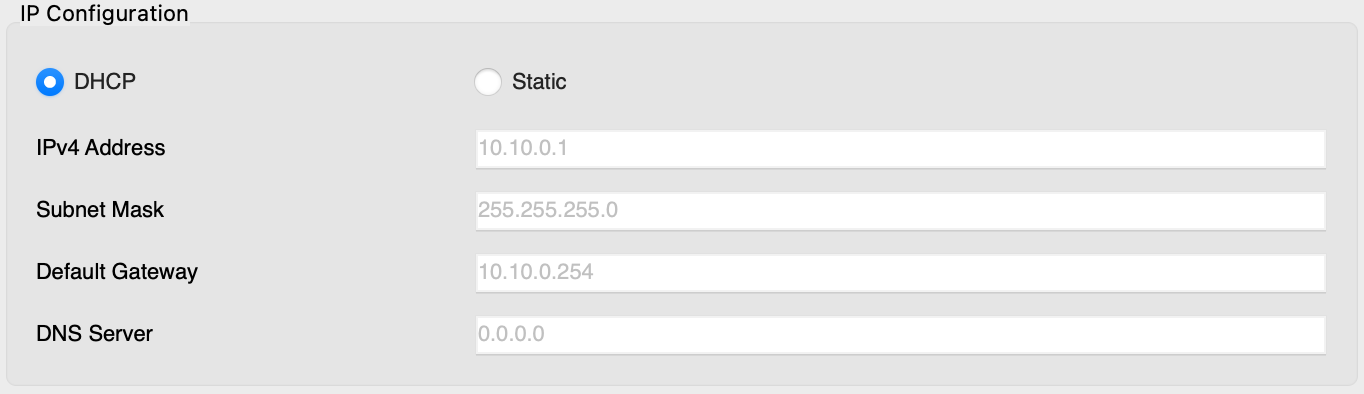
\includegraphics[width=\textwidth]{images/task-2/dhcp-request.png}
  \caption{Получение настроек с помощью DHCP}
  \label{fig:task-2:dhcp-request}
\end{figure}

Так было проделано для всех устройств в сети. После этого нужно было
протестировать доступность устройств, находящихся в том же VLAN, и
недоступность, находящихся в другом VLAN. Для этого с компьютера PC0,
находящийся в первой сети, был сделан ICMP-запрос к PC3, находящийся во второй
сети. В итоге все пакеты были доставлены до адресата (рис.
\ref{fig:task-2:ping-success}). Если попытаться отправить ICMP-запрос с
компьютера PC0, находящемся во VLAN 10, к ноутбуку Laptop3, который находится во
VLAN 50, то запрос не пройдет (рис. \ref{fig:task-2:ping-failed}).

\begin{figure}[H]
  \centering
  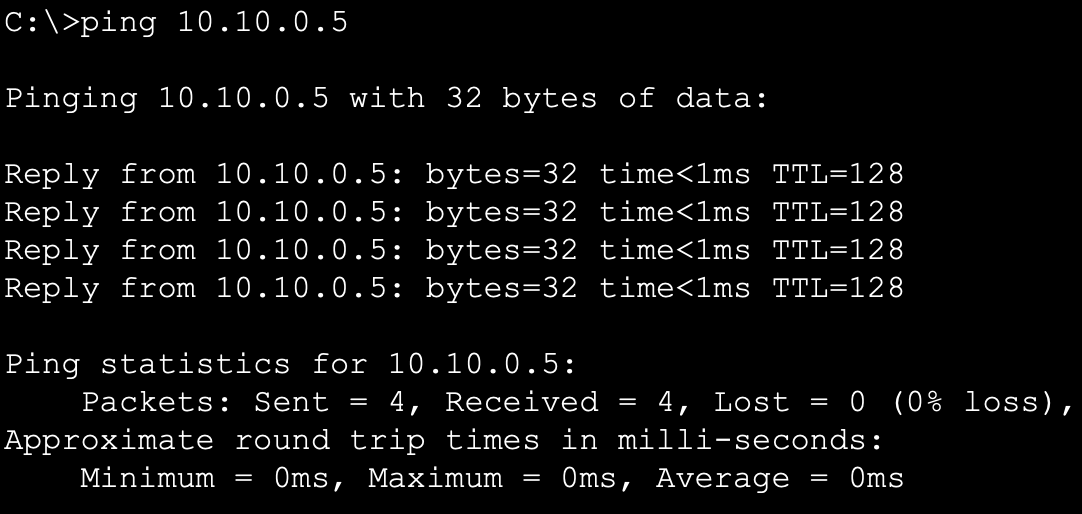
\includegraphics[width=\textwidth]{images/task-2/ping-success.png}
  \caption{Успешный ICMP-запрос от PC0 к PC3}
  \label{fig:task-2:ping-success}
\end{figure}

\begin{figure}[H]
  \centering
  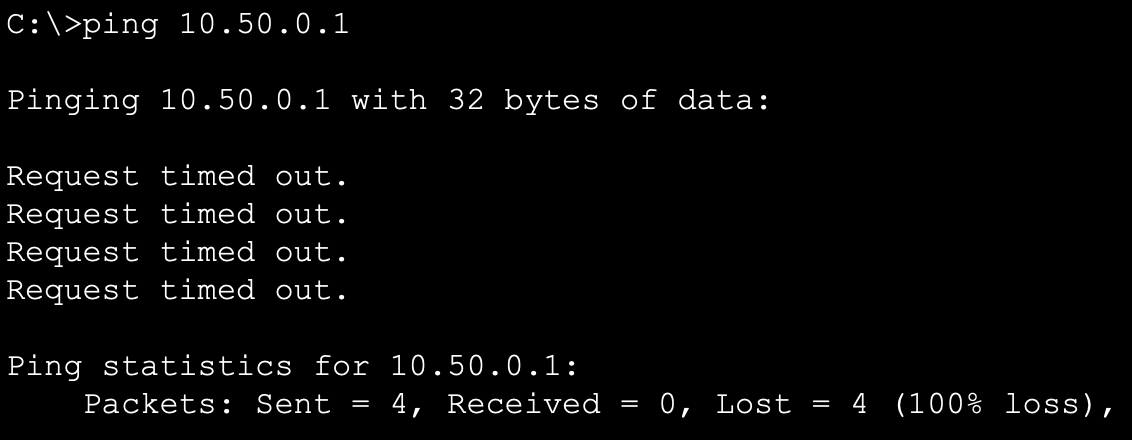
\includegraphics[width=\textwidth]{images/task-2/ping-failed.png}
  \caption{Неудачный ICMP-запрос от PC0 к Laptop3}
  \label{fig:task-2:ping-failed}
\end{figure}

\section{Заключение}

В ходе выполнения данной лабораторной работы я изучил и практически ознакомился
с основными принципами работы концентраторов и коммутаторов второго уровня в
компьютерных сетях, а также настроил и использовал DHCP-сервер для
автоматической выдачи IP-адресов в локальной сети.

\end{document}
